% This file is isea.tex.  It contains the formatting instructions for and acts as a template for submissions to ISEA 2015.  It is based on the ICCC  formats and instructions.  It uses the files isea.sty, isea.bst and isea.bib, the first two of which also borrow from AAAI IJCAI formats and instructions.
% Modified from ICCC.tex by B. Bogart

\documentclass[letterpaper]{article}
\usepackage{isea}
\usepackage[pdftex]{graphicx}
\usepackage{times}
\usepackage{helvet}
\usepackage{courier}
\usepackage[numbers]{natbib}
\usepackage{float}
\pdfinfo{
/Title (Resilient Next-Hop Groups in Linux)
/Author (Netdev 0x15)}
% The file isea.sty is the style file for ISEA 2015 proceedings.
%
\title{Resilient Next-Hop Groups in Linux}
\author{Ido Schimmel, Petr Machata\\
Nvidia\\
idosch@nvidia.org, petrm@nvidia.org\\
\newline
\newline
}
\setcounter{secnumdepth}{0}

\begin{document}
\maketitle
\begin{abstract}
Multipath next-hop groups are used to describe a situation in which it is
possible to forward packets through one of several next hops, each of which
will bring the packet in question closer to the destination. A typical
algorithm to decide which next-hop to forward the packet through is
hash-threshold, whereby a hash derived from packet headers is compared
against hash space ranges assigned to individual next hops. The downside of
this algorithm is that next hop addition, removal, and weight adjustment
may end up redirecting flows that have previously been forwarded to
unrelated next hops. This in turn may cause connection resets and
performance hits. This paper presents resilient next-hop groups, an
approach to hash space management that minimizes incidental hash space
reassignment across next hop additions, removals, and weight adjustments.
\end{abstract}

\section{Keywords}
Linux, ECMP, next-hop groups, resilient hashing

\section{Motivation}

ECMP is typically used in one of two scenarios. To balance traffic between
different paths that all lead to the same destination. Or to balance
traffic between different servers with the same anycast IP address. This is
illustrated by figure ~\ref{fig:ECMP}.

\begin{figure*}[h]
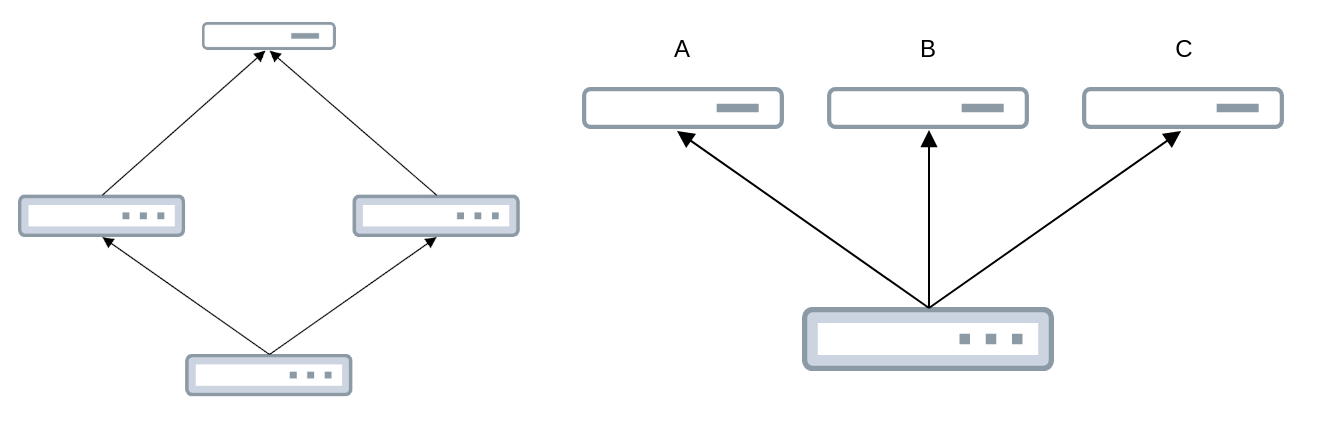
\includegraphics[width=\textwidth]{ECMP.png}
\caption{ECMP use cases. Left: balancing between different paths leading to
  the same server. Right: balancing between servers.}
\label{fig:ECMP}
\end{figure*}

Common strategies when deciding which of the available next hops to forward
the packet through include modulo-N and hash-threshold
algorithms\protect\cite{rfc2992}. In both cases, hash over several packet
fields is first obtained. In the case of modulo-N algorithm, the next hop
to choose is decided simply by applying a modulo-N operation (with N the
number of paths) on the packet hash. In the case of hash-threshold, each
next hop is assigned a contiguous area of the hash space. A packet is then
forwarded through the next hop that contains the packet's hash.

When number of next hops changes, both algorithms change the next hop that
packets with certain hashes would be forwarded to. The amount of this
disruption depends on the algorithm. Under modulo-N, the mapping from
hashes to next hop is just completely different after the number of next
hops changes. Hash-thresholds mitigates this disruption, but is not immune
to it either. Figure ~\ref{fig:hash-threshold-disruption} illustrates what
happens as one next hop is removed.

\begin{figure}[H]
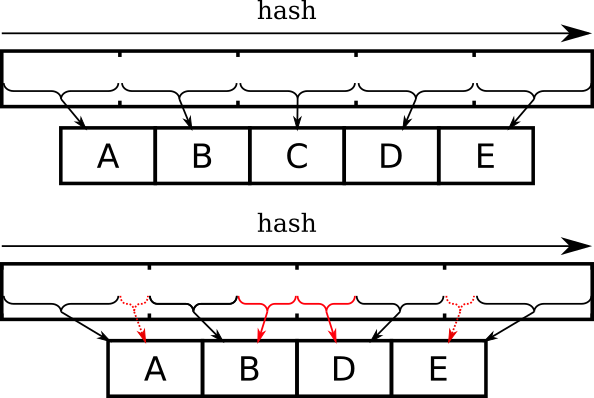
\includegraphics[width=3.31in]{hash-threshold-disruption.png}
\caption{As next hop C is removed, a part of hash space previously assigned
  to B is reassigned to A, and parts of D to E.}
\label{fig:hash-threshold-disruption}
\end{figure}

The disruption outlined above in practice means that certain traffic flows
may get redirected through a different path or to a different server. The
former may lead to packet reordering, which might have performance impacts.
The latter is problematic since an established TCP connection forwarded to
a server that is not familiar with the connection will result in the
connection being reset.

\section{Approach}

The core idea behind resilient next-hop groups is to split the hash space
into regular-sized, but fine-grained buckets, and assign these to next hops
arbitrarily.

By permitting this fine-grained assignment, it is then possible to reassign
only those parts of hash space that it is actually necessary to reassign,
or whose reassignment causes the least disruption. If the granularity is
sufficiently fine it is still possible to model different counts of next
hops with varying weights without introducing errors. And the fact that the
buckets are regular makes the solution manageable in terms of
implementation effort, runtime performance and possible in-HW
implementation.

Next-hop selection algorithm then again becomes modulo-N, except now N
refers to the number of buckets. The next hop to forward through is the one
that this bucket is assigned to. Since the number of buckets is fixed, the
choice of the modulo-N algorithm will not negatively impact the amount of
traffic disruptions. See figure ~\ref{fig:reshash-stable} for illustration.

\begin{figure}[H]
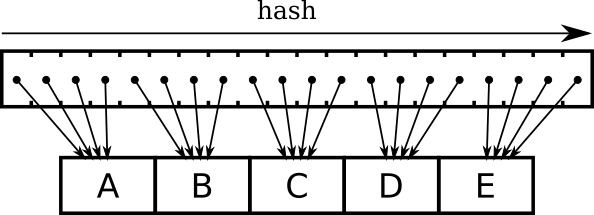
\includegraphics[width=3.31in]{reshash-stable.png}
\caption{Resilient next-hop groups introduce a layer of indirection between
  the hash and the next hops.}
\label{fig:reshash-stable}
\end{figure}

A case where this algorithm works very well is next-hop removal. As a next
hop is removed, any flows hitting that next hop will certainly be
disruptied anyway. Therefore the buckets assigned to the removed next hop
can be freely distributed among the existing next hops according to their
weights. There is no incidental disruption, as the traffic hitting the
buckets assigned to the other next hops keeps getting resolved to the same
next hops as before. This is illustrated in figure
~\ref{fig:reshash-removal}.

\begin{figure}[H]
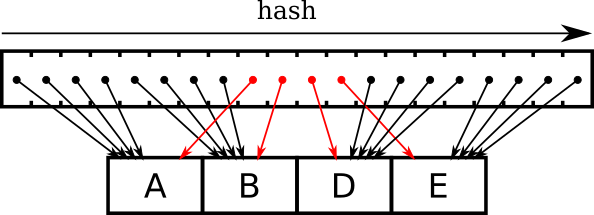
\includegraphics[width=3.31in]{reshash-removal.png}
\caption{As next hop C is removed, its buckets are reassigned to other next
  hops. There is no incidental disruption.}
\label{fig:reshash-removal}
\end{figure}

Next hop addition is a bit more difficult. The issue is that hash space for
the new next hop has to come from somewhere, and there is no other way to
get it but to take from the current next hops. (This is illustrated in
figure ~\ref{fig:reshash-addition}.) The algorithm therefore has no choice
but to disrupt some flows. This is unlike the removal case, where the
choice of which flows to disrupt was imposed by external reality.

\begin{figure}[H]
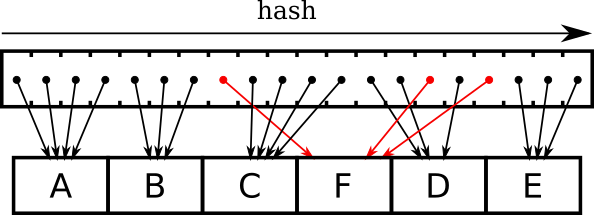
\includegraphics[width=3.31in]{reshash-addition.png}
\caption{As next hop F is added, some buckets must be reassigned from other
  next hops to satisfy F's hash space demands.}
\label{fig:reshash-addition}
\end{figure}

The resilient next-hop algorithm has three-tiered approach to minimizing
this disruption.

The first tier is keeping track of bucket activity. The idea here is that
each bucket knows when it was last used. A system administrator, as they
are configuring the next-hop group, decides after how much time of not
seeing traffic a given bucket is considered idle. Then when choosing which
buckets to reassign, only idle buckets are eligible.

However bucket activity depends on traffic being forwarded, and a
particularly unfortunate pattern could mean that there are no idle buckets
that it makes sense to reassign. That is when the second tier comes into
play. In that situation the algorithm will back off for a while, and will
attempt to reassign buckets later.

Obviously the situation may be such that there keep being no idle buckets
to reassign. The third tier is a possibility to force-balance the next-hop
group. In that case the resilient group can be configured to reassign
buckets without regard to their idleness.

\section{Algorithm}

In a nutshell, the algorithm works as follows. Each next hop deserves a
certain number of buckets, according to its weight and the number of
buckets in the hash table. In accordance with the source code, we will call
this number a \emph{wants count} of a next hop. In case of an event that
might cause bucket allocation change, the wants counts for individual next
hops are updated.

Next hops that have fewer buckets than their wants count, are called
\emph{underweight}. Those that have more are \emph{overweight}. If there
are no overweight (and therefore no underweight) next hops in the group, it
is said to be \emph{balanced}.

Each bucket maintains a last-used timer. Every time a packet is forwarded
through a bucket, this timer is updated to current jiffies value. One
attribute of a resilient group is then the \emph{idle timer}, which is the
amount of time that a bucket must not be hit by traffic in order for it to
be considered \emph{idle}. Buckets that are not idle are busy.

After assigning wants counts to next hops, an \emph{upkeep} algorithm runs.
For buckets:

\begin{itemize}
\item that have no assigned next hop, or
\item whose next hop has been removed, or
\item that are idle and their next hop is overweight,
\end{itemize}

upkeep changes the next hop that the bucket references to one of the
underweight next hops. If, after considering all buckets in this manner,
there are still underweight next hops, another upkeep run is scheduled to a
future time.

There may not be enough \emph{idle} buckets to satisfy the updated wants
counts of all next hops. Another attribute of a resilient group is the
\emph{unbalanced timer}. This timer can be set to 0, in which case the
table will stay out of balance until idle buckets do appear, possibly
never. If set to a non-zero value, the value represents the period of time
that the table is permitted to stay out of balance.

With this in mind, we update the above list of conditions with one more
item. Thus buckets:

\begin{itemize}
\item whose next hop is overweight, and the amount of time that the table
  has been out of balance exceeds the unbalanced timer, if that is
  non-zero,
\end{itemize}

... are migrated as well.

\section{Implementation}

In Linux 5.3, support for standalone next-hop objects has been added to the
Linux kernel. Resilient next-hop groups have been implemented as a new
next-hop group type.

\section{User Interface}

The fact that resilient next-hop groups are implemented on top of the
standalone next-hop objects informs how the \texttt{iproute2} CLI will look
like. A new \texttt{type} keyword has been added to the nexthop group suite
of commands. When type is \texttt{resilient}, a number of parameters to
configure the resilient-specific attributes of the next-hop group can be
specified. For example:

\begin{verbatim}
# ip nexthop add id 1 via 192.0.2.2 \
     dev dummy1
# ip nexthop add id 2 via 198.51.100.2 \
     dev dummy2
# ip nexthop add id 10 group 1/2 \
     type resilient buckets 8 \
     idle_timer 120 unbalanced_timer 300
\end{verbatim}

... first creates two next hops, and then groups them in a resilient group.
\texttt{buckets} refers to number of buckets (and therefore hash space
assignment granularity). The size of 8 indicated here is probably too low
and is used for illustration purposes only. Typically one wants
approximately hundreds of buckets, so that different counts of next hops
and various odd weight ratios can be modeled accurately.

\texttt{idle\_timer} and \texttt{unbalanced\_timer} are discussed above.

Individual parameters (except for the number of buckets, which is fixed)
can be changed. E.g. in the following, only, respectively,
\texttt{idle\_timer} and \texttt{unbalanced\_timer} are adjusted, with the
other staying intact:

\begin{verbatim}
Change attributes of the group
# ip nexthop replace id 10 group 1/2 \
     type resilient idle_timer 100
# ip nexthop replace id 10 group 1/2 \
     type resilient unbalanced_timer 900
\end{verbatim}

Of particular interest is then that in neither of these cases, any bucket
reassignments are done. The bucket table stays intact. Likewise in the
following:

\begin{verbatim}
# ip nexthop replace id 10 \
     group 1,9/2,11 type resilient
\end{verbatim}

Here we have changed the weights of the next hops. But as explained above,
that does not by itself change any bucket reassignments. Instead the group
becomes unbalanced, because next hop 1 now has more buckets than it should
have, and next hop 2 has fewer. Then the upkeep algorithm gradually brings
the group into balance (or not, depending on the configuration).

In is obviously possible to dump the group as well:

\begin{verbatim}
# ip nexthop show id 10
id 10 group 1/2 type resilient
buckets 8 idle_timer 60
unbalanced_timer 300 unbalanced_time 0
\end{verbatim}

The \texttt{unbalanced\_time} (as opposed to \texttt{unbalanced\_timer})
shows the amount of time that the group has been out of balance. The 0
indicated here means that the group is actually balanced.

Finally, the netlink API has been extended with a new message type,
\texttt{RTM\_GETNEXTHOPBUCKET}, to dump individual buckets. That API is
implemented in \texttt{iproute2}, too, and thus it is possible to
introspect the state of the bucket table:

\begin{verbatim}
# ip nexthop bucket show id 10
id 10 index 0 idle_time 5.59 nhid 1
id 10 index 1 idle_time 5.59 nhid 1
id 10 index 2 idle_time 8.74 nhid 1
id 10 index 3 idle_time 8.74 nhid 1
id 10 index 4 idle_time 8.74 nhid 2
id 10 index 5 idle_time 8.74 nhid 2
id 10 index 6 idle_time 8.74 nhid 2
id 10 index 7 idle_time 8.74 nhid 2
\end{verbatim}

(And now you know why the group only has 8 buckets.)

\section{Offloading}

Resilient next-hop groups are not novel, in fact the algorithm is commonly
implemented in SDKs for networking switches and routers. The fact that it
has not been implemented in the software datapath so far perhaps indicates
that it is less critical in software-only deployments. It is therefore
important to make it possible to implement offloading of resilient next-hop
groups.

The resilient algorithm hinges on the fact that it understands which next
hop buckets are idle. In software datapath, this understanding is achieved
by maintaining per-bucket last-used time. However, when accelerating
traffic by offloading to capable devices, the vast majority of traffic is
never seen by the algorithm.

A two-pronged approach is implemented to close this loophole.

First, as is usual, the core next-hop algorithm communicates information
about the events in resilient next-hop groups using the in-kernel
notification mechanism. Bucket migration notifications in particular are of
two flavors: forced and vetoable. Forced notifications are used if a next
hop is removed and the algorithm simply needs to migrate a given bucket to
another next hop. Vetoable notifications are used for the regular table
upkeep, as the algorithm finds new idle buckets and proposes them for
migration. The idea is that a driver will take note of these proposals, and
in turn will propose them to the device, which may bounce them if hardware
datapath traffic has been using the bucket in question.

The second prong is a proactive reporting by the driver towards the
next-hop code. A new in-kernel API
\texttt{nexthop\_res\_grp\_activity\_update()} can be called to feed an
activity bit vector from the device to the next-hop group. Set bits in the
vector are treated as if software-datapath traffic hit the corresponding
bucket.

\begin{figure}[H]
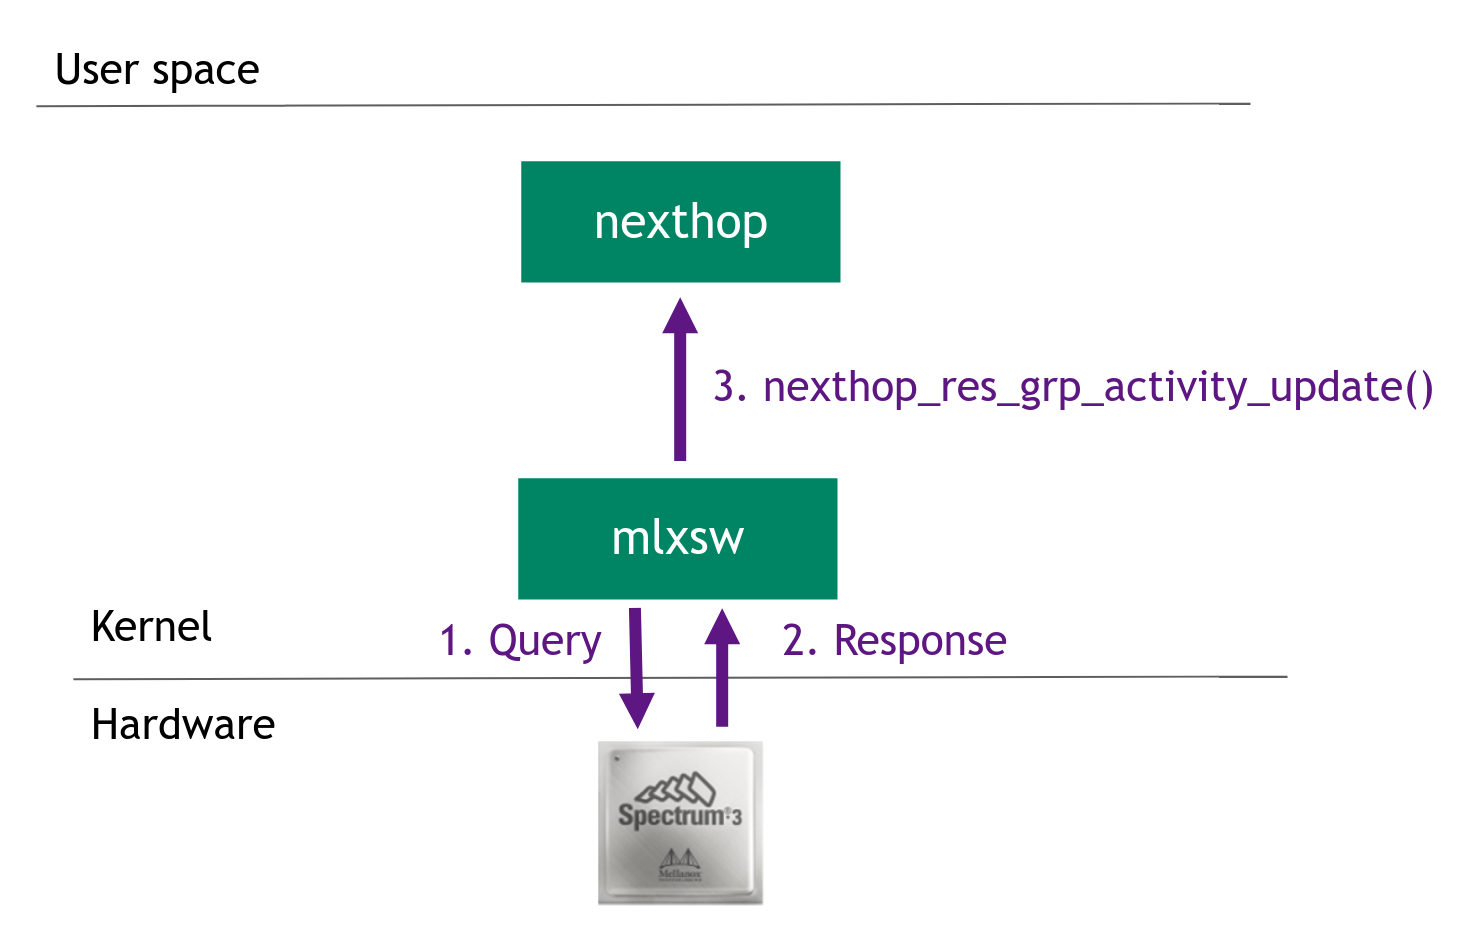
\includegraphics[width=3.31in]{nexthop_res_grp_activity_update.png}
\caption{Driver periodically calls
  \texttt{nexthop\_res\_grp\_activity\_update()} to keep bucket activity up
  to date.}
\label{fig:nexthop_res_grp_activity_update}
\end{figure}

The notification-based approached would be enough to implement the raw
functionality. However, it would inevitably lead to a lot of ping-pong
between the core next-hop code, the driver and the device, as the algorithm
would keep proposing migrations that involved busy buckets. Reporting
through the new API makes sure that the core has a reasonable idea of what
is going on in the device. At the same time, the notification-based
approach is necessary to close the race between the driver report and new
hardware datapath flows popping up and making a bucket busy.

\subsection{Bucket Flags}

As individual buckets are offloaded (or configured to trap traffic to
software datapath), a driver ought to mark them with either
\texttt{offload} or \texttt{trap} flags.

\section{Testing}

A number of selftests have been added in order to check that the algorithm
behaves in an expected manner. Specifically for testing edge cases of the
bucket migration algorithm, faux \texttt{netdevsim} offload has been added.

The module exposes a debugfs interface that allows marking individual
buckets as busy. For example, to mark bucket 23 in next-hop group 10 as
active, one would write the string ``10 23'' to file
\texttt{/sys/kernel/debug/netdevsim\\/netdevsimX/fib/nexthop\_bucket\_activity}.
Another interface, \texttt{\ldots/fib/fail\_nexthop\_bucket\_replace},
allows configuring that the next attempt to migrate a bucket should fail.

These interfaces permit careful testing of the algorithm edge cases. It is
for example possible to keep busy the buckets that belong to certain next
hops, then lower that next hop's weight, and observe how the algorithm
handles the transition.

\bibliographystyle{isea}
\bibliography{isea}

\end{document}
